\documentclass{scrbook}
\usepackage{indentfirst}
\usepackage{tikz}
\usepackage{amsmath}
\usepackage{pgfplots}
\usepackage[backend=bibtex]{biblatex}
\addbibresource{Physics.bib}
\title{Physics Notes}
\subtitle{A level Physics}
\date{Last Updated \today{}}
\author{Dhruva Lokegaonkar}
\begin{document}
\maketitle
\tableofcontents
\chapter{Circular Motion, Gravitation and Oscillation}

\section{Circular Motion}

\subsection{Measurement}
	Angles or angular displacement is usually measured in radians. $360^\circ = 2\pi rad$

	\begin{quote}
		One Radian is the angle subtended at the center of a circle by an arc of length equal to the radius of the circle
	\end{quote}

	The time period of rotation is $T$ and frequency is $f$

	\[ \omega = \frac{2\pi}{T} = 2\pi f \]

\subsection{Angular Velocity and Centripetal Force}

	The speed at which a object rotates is called it's angular velocity. It is measured in $rad\ s^{-1}$ and is represented by $\omega$. This is different from it's linear velocity.
	
	\begin{align*}
	\omega = \frac{\Delta \theta}{\Delta t} & & v = \omega r
	\end{align*}

	Even if a rotating object has constant angular velocity, it's linear velocity is not constant. This is because velocity is a vector and an object in circular motion is constantly changing direction. Since there is a change in velocity, there is acceleration. This acceleration is called centripetal acceleration. It can be calculated using a vector diagram.
	
	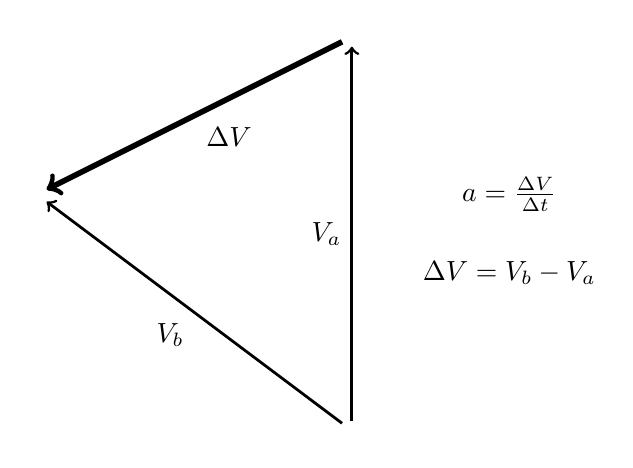
\begin{tikzpicture}[node distance=25mm]
		\node (a) at (0, 0) {};
		\node (b) at (0, 5) {};
		\node (c) at (-4, 3) {};

		\node (eqn) at (2, 3) {};
		\draw (eqn) node {$a = \frac{\Delta V}{\Delta t}$};

		\node (delv) at (2, 2) {};
		\draw (delv) node {$\Delta V = V_b - V_a$};

		\draw[->, line width=1pt] (a) to node[auto] {$V_a$} (b);
		\draw[->, line width=1pt] (a) to node[auto] {$V_b$} (c);
		\draw[->, line width=2pt] (b) to node[auto] {$\Delta V$} (c);
	\end{tikzpicture} 

	The Centripetal acceleration is due to centrepetal forces, which can be gravity or tension in a string. This can be calculated by $F = ma$. Centrepetal acceleration can also be calculated by the follwing formulas: $a = v\omega$, $a = \frac{v^2}{r}$, and $a = \omega ^2 r$. Multiplying by mass gives $F = mv\omega$, $F = \frac{mv^2}{\omega}$, and $F = m\omega^2r$

\section{Gravitation}

\subsection{Newton's Law of Gravitation}

	\begin{quote}
		Any two point masses attract each other with a force that is directly proportional to the product of their masses and inversely proportional to the square of the seperation.
	\end{quote}

	Newtons law can be summaried in the folling equations.
	
	\begin{align*}
		\text{force} &\propto \text{product  of  masses} &
		\\
		\text{force} &\propto \frac{1}{\text{distance}^2} &
		\\
		F &= \frac{GMm}{r^2} & \text{Introducing the constant G, where } G = 6.67\times 10^{-11} Nm^2kg^{-2}
	\end{align*}

\subsection{Gravitational Field Strength}

	\begin{quote}
		The gravitational field strength at a point is the gravitational force exerted per unit mass on a object at a poiny
	\end{quote}

	This is represented by $g$

	\begin{align*}g = \frac{F}{m} & & g = \frac{GM}{r^2}\end{align*}
	
\subsection{Gravitational Potential}

	\begin{quote}
		The gravitational potential at a point is the work done per unit mass to bring a abject from inifinty to a point
	\end{quote}

	It is zero at infinity and negative at any point in the universe. It is represented by the greek letter $\phi$ (phi) and is calculated using the following formula

	\[ \phi = \frac{-GM}{r} \]

\subsection{Orbiting Under Gravity}

	The equations of circular motion and gravitation can be combined to give the equation for orbits under gravity

	\[ F = \frac{mv^2}{r} = \frac{GMm}{r^2}\]
	\[ \text{so } v^2 = \frac{GM}{r}\]

	For an object in a geostationary orbit, the time period can be calculated by using the folling formula

	\[ T^2 = \left(\frac{4\pi^2}{GM}\right)r^3 \]

\section{Oscillations}

	Oscillations or vibrations are to and fro motions. They have three key properties: Frequency, amplitude and period

\subsection{Phase}

	Phase describes the point that an oscillating mass has reached within the complete cycle of an oscillation. It is often measured in degrees or radians. 

\subsection{Simple Harmonic Motion (s.h.m.)}

	There are three requirements for a mechanical system to be in s.h.m:

	\begin{itemize}
		\item
			A mass that oscillates
		\item
			A position where the mass is in equilibrium 
		\item
			A restoring force that acts to return the mass to it's equilibrium position.
	\end{itemize}

	The force is directly proportional to the displacement from the equilibrium position. The following equations describe s.h.m for a oscillator which is at the equilibrium position at $t = 0$

	\begin{align*}
		x &= x_0\sin{\omega t}
		\\
		v &= v_0\cos{\omega t}
		\\
		a &= -\omega^2x
		\\
		v &= \pm \omega \sqrt{x_0^2 - x^2}
		\\
		v_{max} &= \omega x_0
	\end{align*}

\subsection{Resonance and Damping}

	Resonance is a phenomenon observed in systems with forced oscillations. The following statements apply to systems in resonance

	\begin{itemize}
		\item
			It's natural frequency is equal to the frequency of the driver.
		\item
			It's amplitude is maximum
		\item
			It absorbs the greatest possible energy from the driver.
	\end{itemize}

	Damping is when a oscillating system loses energy (due to friction or air resistance). Critical Damping is minimum amount of energy required to return a damped system to equilibrium without oscillating

\chapter{Communication Systems}

\section{Modulation}

\subsection{F.M. and A.M.}

	When sending information over radio waves, the information must be modulated in some way. A common way of mudulating is Amplitude Modulation or AM. We can see in Fig \ref{fmamcomp} that the amplitude of the modulated wave changes to match the value of the signal. In Frequency Modulation or F.M. the frequency of the modulated wave varies with time. Example can be seen in Fig \ref{fmamcomp}

	\begin{figure}[t]
		\caption{Comparison of FM and AM \cite{taitra}}
		\label{fmamcomp}
		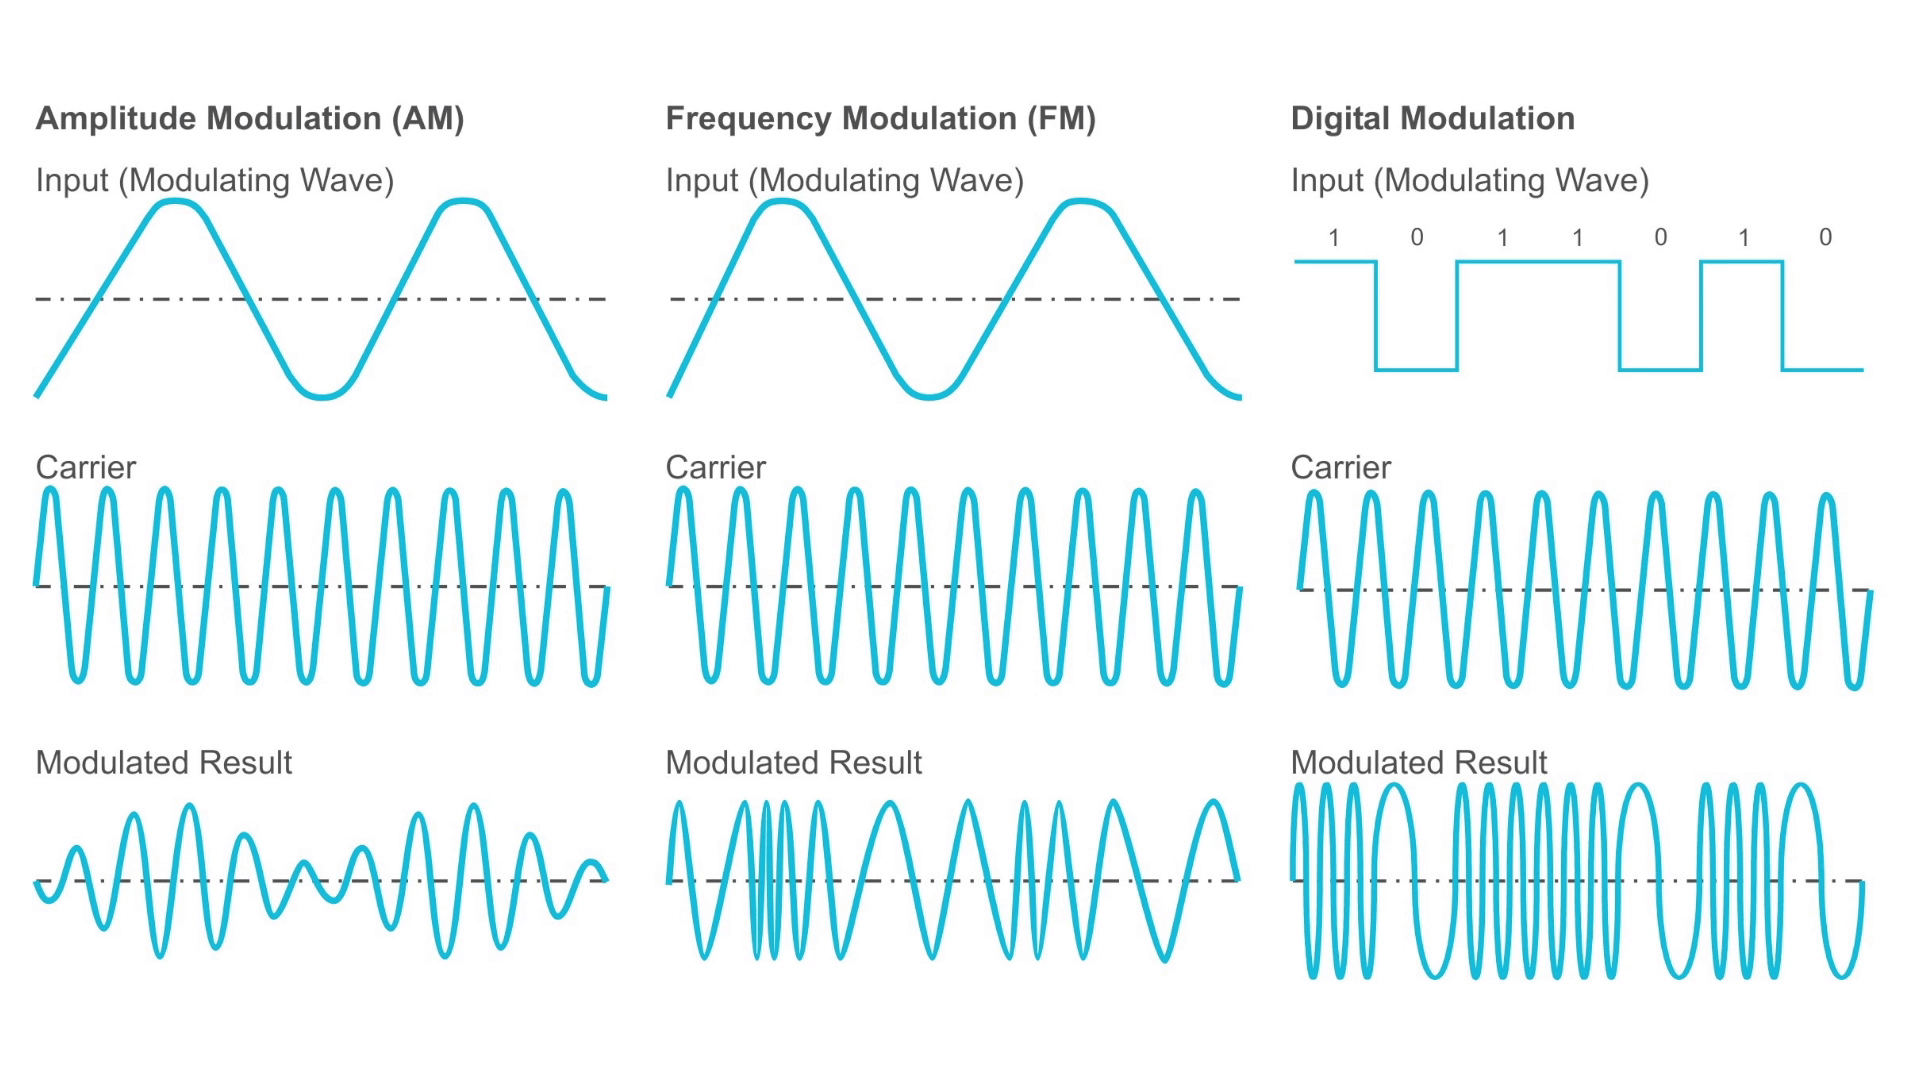
\includegraphics[width=\linewidth]{assets/fmam.png}
	\end{figure}

\subsection{Sidebands and Bandwidth}

	The frequency of the carrier wave is known as the carrier frequecny ($f_c$). When the carrier wave is modulated, it is known to carry two more frequencies called Sideband frequencies ($f_c - f_m$ and $f_c + f_m$). The bandwidth is $2f_m$

\subsection{Comparison}

	\begin{tabular}{| c | c |}
		\hline
		FM & AM \\
		\hline
		Less Electrical Interference and Noise & Greater area covered by one transmitter \\
		Greater bandwidth produces better sound & Smaller bandwidth allows for more stations \\
		& Cheap Radio Sets \\
		\hline
	\end{tabular}

\section{Digtal Signals}

\subsection{Advantages of Digital signals}

	\begin{itemize}
		\item
			Noise can be fixed through regeneration.
		\item
			Digital Signals are more compatible with modern technologies
		\item
			Digital electronic systems are more reliable, robust and easier to build.
		\item
			Digital signals build in safegaurds so that if there is an error in recepotions, the required parts of the signal can be sent again.
	\end{itemize}

\subsection{ADC, DAC and Sampling}

	When converting between analigue and digital signals, signals must be sampled at regular intervals. The rate at which it is sampled is called the Sample Rate. The resoultion at which the signal is sampled is called the bit-depth


\section{Crosstalk and Signal Attenuation}

	\begin{quote}
		Crosstalk or Crosslinking occurs when a signal transmitter in one circuit or channel creates an undesired effect in another circuit or channel
	\end{quote}

	\begin{quote}
		Signal Attenuation is the gradual decrease in power of a signal the further it travels.
	\end{quote}

	The decrease in power from $P_1$ to $P_2$ can be very high. A $\log_{10}$ is used and the ratio is reprented in Bels (often multiplied by 10 and written as deciBels or dB)

	\[ \text{Attenuation}  = 10\log_{10}\left(\frac{P_1}{P_2}  \right) \text{dB}\]

\section{Channels of Communications}

\subsection{Wire Pairs and Co-axial cables}

	Telephones used to use pairs of wires to carry signals. The difference in the Potential differences of the wires was the signal, but they easily picked up noise. The closer the wires were, the less noise was picked up, so they were twisted together.

	Coaxial reduces the amount of crosstalk in the wire when the transmission occurs at high speeds. The copper core usually carries the signal and the copper braid (mettalic shield) is connected to earth. see Fig \ref{coaxial} Since electromagnetic radiation does not travel easily through metal, inteference does not occur at the core.

	\begin{figure}[t]
		\label{coaxial}
		\caption{A Coxial Cable \cite{wikicomm:coax}}
		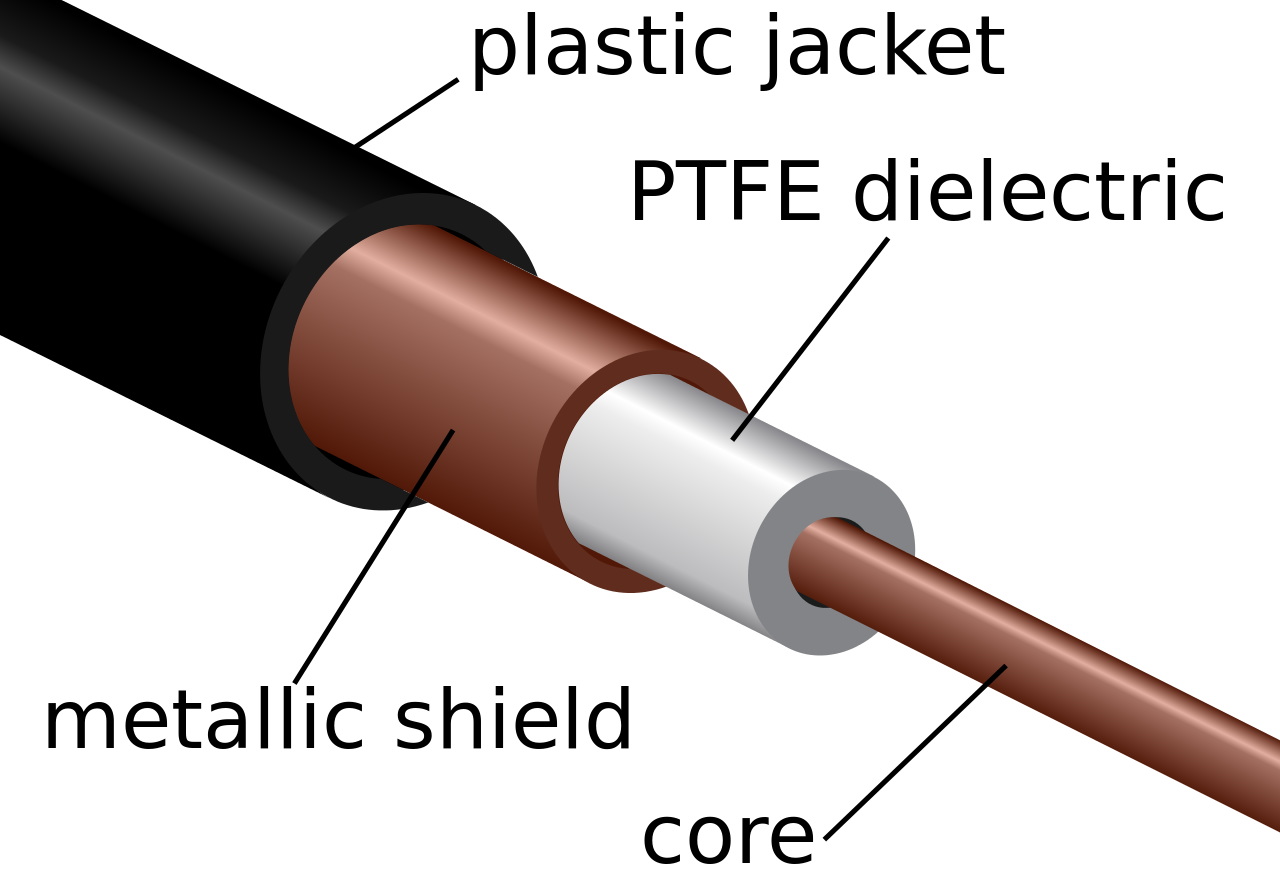
\includegraphics[width=\linewidth]{assets/coaxial.png}
	\end{figure}

	\begin{tabular}{| c | c |}
		\hline
		Wire Pairs & Coaxial \\
		\hline
		Cheap and convenient & Expensice \\
		Strongly attenuate signal & Less attenuating \\
		Low bandwidth & High bandwidth \\ 
		Pushes up inteference/noise & Less inteference and noise \\
		Crosstalk & less Crosstalk \\
		Low security & More secure \\
		\hline
	\end{tabular}

\subsection{Radio Waves and Microwave links}

	Various electromagnetic waves are used to carry informations. In waves such as skywaves, the ionosphere is used to reflect the waves.

	\begin{tabular}{| c | c | c |}
		\hline
		Type & Frequency Range & Distance Travelled \\
		\hline
		Surface wave & upto 3MHz & upto 1000Km \\
		Sky wave & 3 - 30MHz & Worldwide by reflection \\
		Space wave & 30 - 300MHz & line of sight \\
		Microwave & 1-300GHz & line of sight, except when retransmitted by sattelite \\
		\hline
	\end{tabular}

\subsection{Sattelites and Optic fibre}

	Sattelites offer some extra advantages over skywaves

	\begin{itemize}
		\item
			The concentration of ions in the ionosphere is constantly changing and the reflection of skywaves is not always possible
		\item
			The sattelite boosts the signal for its return to earth.
		\item
			Sattelite communications use higher frequencies and hence have height bandwidth
		\item
			More channels are available for communicating on higher frequencies
	\end{itemize}:q


\printbibliography{}

\end{document}
